\section{Struktogramme}
Beim Programmieren ist es häufig hilfreich, sich vorab die Zeit zu nehmen und das Programm durchzuplanen, bevor mit der eigentlichen Programmierung angefangen wird. Um Programme zu planen existiert eine Vielzahl an grafischen Modellierungshilfen. Diese sind dazu da, Programmaufbau und Ablauf in grafischer Form übersichtlich darzustellen. Eine Möglichkeit hierfür sind so genannte Struktogramme (auch Nassi-Schneiderman Diagramme). \\
Das Diagramm besteht aus verschiedenen Elementen, welche die Elemente eines Programms widerspiegeln. Für uns sind zunächst die von Python unterstützen Elemente interessant.

\begin{figure}[H]
	\begin{center}
		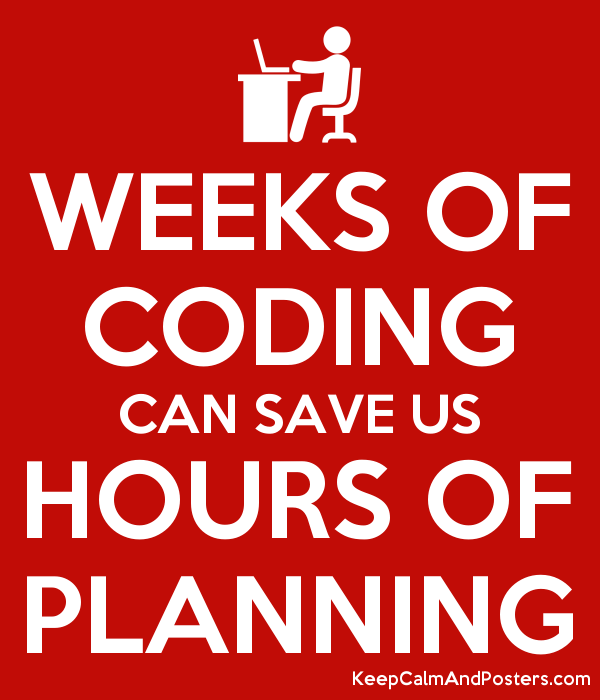
\includegraphics[width=0.4\textwidth]{imgs/weeks_coding.png} % Include the image placeholder.png
		\caption{Weeks of coding...}
	\end{center}
\end{figure}

\subsection{Symbolik} \label{sec:Symbolik}
\subsubsection{Anweisung}
Eine Anweisung wird in einem rechteckigen Kasten geschrieben. Alle die Blöcke werden von oben nach unten abgearbeitet. Im folgenden Beispiel wird der Betrag einer Zahl berechnet und ausgegeben, welche zuvor eingelesen wurde.\\

\begin{minipage}{.45\textwidth}
\centering
\begin{figure}[H]
	\begin{center}
		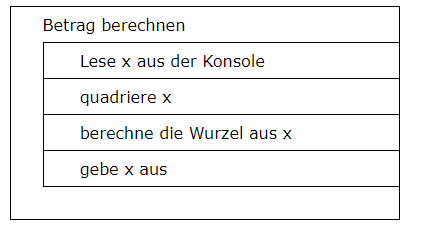
\includegraphics[width=0.9\textwidth]{imgs/abs_long.png} % Include the image placeholder.png
	\end{center}
\end{figure}
\end{minipage}
\begin{minipage}{.45\textwidth}
\begin{python}
from math import sqrt

x = int(input("x eingeben: "))
x = x**2
x = sqrt(x)
print(x)
\end{python}
\end{minipage}
\subsubsection{If-Abfrage}

Eine If-Abfrage\footnote{Achtung: Es wird IF-Abfrage genannt. If-Schleifen gibt es nicht!!!} stellt eine Verzweigung im Programm dar. Wir lesen eine Zahl ein. Falls die Zahl negativ ist, soll der Betrag berechnet werden. Abschließend wird die Zahl ausgegeben:\\

\begin{minipage}{.45\textwidth}
\centering
\begin{figure}[H]
	\begin{center}
		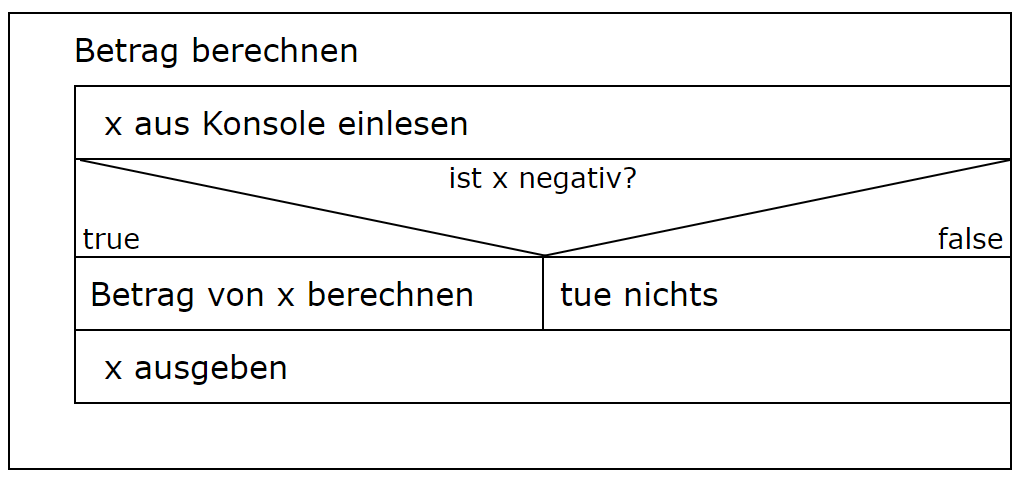
\includegraphics[width=0.9\textwidth]{imgs/if_clause.png} % Include the image placeholder.png
	\end{center}
\end{figure}
\end{minipage}
\begin{minipage}{.45\textwidth}
\begin{python}
x = int(input("x eingeben: "))
if x < 0:
	x = abs(x)
print(x)
\end{python}
\end{minipage}

\subsubsection{For-Schleife}
Wie nehmen an, dass in einer liste eine menge an zahlen steht. Die For-Schleife soll die Zahlen aufsummieren. Abschließend soll die Summe ausgegeben werden:

\begin{minipage}{.45\textwidth}
	\centering
	\begin{figure}[H]
		\begin{center}
			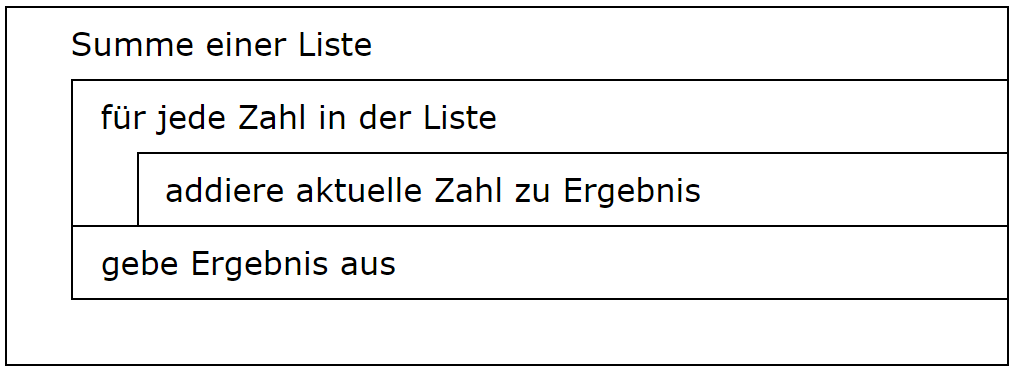
\includegraphics[width=0.9\textwidth]{imgs/for_loop.png} % Include the image placeholder.png
		\end{center}
	\end{figure}
\end{minipage}
\begin{minipage}{.45\textwidth}
\begin{python}
num_lst = [1, 2, 3, 4, 5]
res = 0
for num in num_lst:
	res = res + num
print(num)
\end{python}
\end{minipage}

\subsubsection{While-Schleife}


\subsection{Aufgaben}
Die folgenden Aufgaben könnt ihr mit Hilfe des Tools \textit{structorizer} (https://www.structorizer.com/struct.php) bearbeiten. Das Tool weist weitere Elemente für Struktogramme auf, die wir entweder nicht verwenden oder die nicht in Python vorhanden sind.

\subsubsection{Warmup}
Um warm zu werden mit dem Tool, sollt ihr zunächst die Struktogramme aus \ref{sec:Symbolik} nachbauen. 

\subsubsection{Code zu Struktogramm}
Erstellt aus eurem Code für die Aufgabe 2 (Dinge mit Listen und Schleifen) ein Struktogramm.

\subsubsection{Struktogramm zu Code}
Erstellt zu folgendem Struktogramm das Programm:
\begin{figure}[H]
\begin{center}
	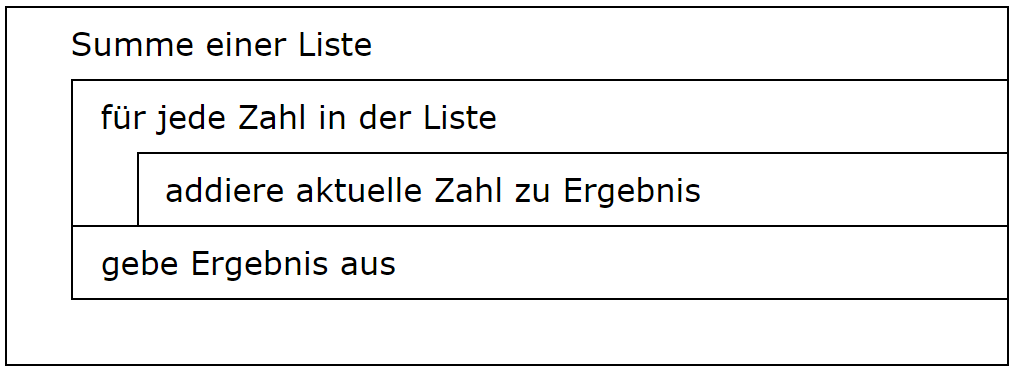
\includegraphics[width=0.9\textwidth]{imgs/for_loop.png} %TODO: passendes Struktogramm
\end{center}
\end{figure}

\subsubsection{Würfeln}
Es soll ein Programm entworfen werden, welches einen Würfel so lange würfelt, bis eine Zahl 3 mal hintereinander gefallen ist. Die Anzahl der benötigten Würfe ist am Ende auszugeben. Der Würfel hat 6 Seiten. \\
Erstellt zunächst das Struktogramm und implementiert eure Lösung anschließend.


\subsubsection{Zahlenspiel}
Ihr sollt ein kleines Zahlenspiel planen und implementieren. Das Spiel wird über die Konsole gespielt. Der Spieler muss eine Zahl (ganze Zahl) erraten, die der Computer sich zuvor ausdenkt. Hierbei wird die vom Spieler geratene Zahl über die Konsole eingelesen. Der Computer gibt daraufhin den Tipp, ob die geratene Zahl kleiner oder größer ist als die zu erratende Zahl. Sollte der Spieler die Zahl richtig erraten, wird das Programm mit einer passenden Ausgabe beendet.\\
Erstellt zunächst das Struktogramm des Spiels. Anhand dieses Struktogramms sollt ihr anschließend das Programm implementieren.